\documentclass[conference]{IEEEtran}
\IEEEoverridecommandlockouts
% The preceding line is only needed to identify funding in the first footnote. If that is unneeded, please comment it out.
\usepackage{cite}
\usepackage{amsmath,amssymb,amsfonts}
\usepackage{algorithmic}
\usepackage{graphicx}
\usepackage{textcomp}
\usepackage{xcolor}
\usepackage{parskip}
\def\BibTeX{{\rm B\kern-.05em{\sc i\kern-.025em b}\kern-.08em
    T\kern-.1667em\lower.7ex\hbox{E}\kern-.125emX}}
\begin{document}

\title{Malware Classification and Detection Using XceptionNet}

\author{\IEEEauthorblockN{Om Gatade}
\IEEEauthorblockA{
\textit{KIT's College of Engineering}\\
\textit{(Autonomous)}\\
Kolhapur, Maharashtra, India \\
omgatade974@gmail.com}
\and
\IEEEauthorblockN{Aseem Athale}
\IEEEauthorblockA{
\textit{KIT's College of Engineering}\\
\textit{(Autonomous)}\\
Kolhapur, Maharashtra, India \\
athaleaseem@gmail.com}
\and
\IEEEauthorblockN{Mahesh Wadhe}
\IEEEauthorblockA{
\textit{KIT's College of Engineering}\\
\textit{(Autonomous)}\\
Kolhapur, Maharashtra, India \\
maheshinkit@gmail.com}
\and
\IEEEauthorblockN{Kedar Salunkhe }
\IEEEauthorblockA{
\textit{KIT's College of Engineering}\\
\textit{(Autonomous)}\\
Kolhapur, Maharashtra, India \\
kedarsalunkhe325@gmail.com}

\and
\IEEEauthorblockN{Dr. Uma P. Gurav}
\IEEEauthorblockA{
\textit{KIT's College of Engineering}\\
\textit{(Autonomous)}\\
Kolhapur, Maharashtra, India \\
gurav.uma@kitcoek.in}

}


\maketitle

\begin{abstract}
Malicious software, or malware, continues to pose a significant threat to computer systems. Traditional antivirus software struggles to keep pace with the evolving nature of malware threats. This research investigates the potential of employing a Convolutional Neural Network (CNN) model for malware classification. The CNN model was trained on a dataset of malware samples represented as grayscale images. The evaluation results demonstrated that the model achieved promising performance in differentiating between various malware classes, exhibiting accuracy superior to a traditional antivirus software in most cases. Additionally, the CNN model offered faster detection times for malware classification compared to traditional methods. These findings highlight the potential of CNN-based approaches for malware classification. However, limitations such as the reliance on the quality and comprehensiveness of the training data exist. Future research directions include exploring more sophisticated CNN architectures, incorporating techniques to address class imbalance, and investigating methods to enhance the model's generalizability to unseen malware variants, along with improving its resilience against adversarial samples.
\end{abstract}

\begin{IEEEkeywords}
Malware classification,
Convolutional Neural Networks (CNNs),
Deep learning,
Image classification,
PE executables
\end{IEEEkeywords}

\section{Introduction}
The ever-growing threat landscape necessitates robust and adaptable methods for malware detection. Malicious software, constantly evolving to bypass traditional antivirus software, disrupts data security, system functionality, and financial well-being. Traditional approaches, often relying on signature-based detection (refer to specific slide number if applicable) or heuristic analysis (refer to specific slide number if applicable), struggle to keep pace with the rapid development of novel malware strains designed to evade such mechanisms.

Deep learning has emerged as a powerful tool in various fields, including cybersecurity. Deep learning algorithms excel at learning complex patterns from vast amounts of data. Convolutional Neural Networks (CNNs), a specific type of deep learning architecture, have achieved remarkable success in image classification tasks. Their ability to automatically extract and learn discriminative features from images makes them well-suited for applications where visual representations play a key role.

This research investigates the potential of employing a CNN model for malware classification. By leveraging the image recognition capabilities of CNNs, this approach aims to develop a more robust and adaptive method for detecting malicious software. We hypothesize that by converting malware samples into grayscale images (refer to specific slide number if applicable) and training the CNN model on a diverse dataset of malware and benign samples, the model can learn to differentiate between malicious and legitimate software with high accuracy.


\begin{figure}[ht] % 'h' stands for 'here', it tries to place the figure here
  \centering % Centers the figure horizontally
  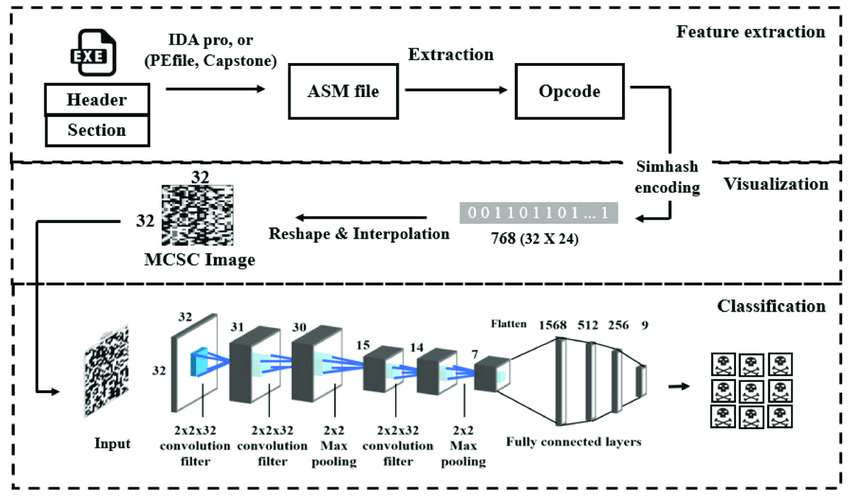
\includegraphics[width=0.5\textwidth]{The-overall-procedure-of-malware-classification-using-Simhash-and-CNN-MCSC-algorithm.png} % Replace 'example-image' with your image filename
  \caption{Executable to Image Conversion Process Demonstration } % Caption for the figure
  \label{fig:example} % Label to refer to the figure in the text
\end{figure}




The remainder of this paper will delve into the methodology employed for training and evaluating the CNN model for malware classification. We will discuss the details of the dataset used, the pre-processing techniques applied to convert malware samples into a suitable format (refer to specific slide number if applicable), and the specific CNN architecture chosen for this research. The results section will present the evaluation metrics employed and the performance achieved by the model in differentiating between various malware classes. We will then analyze the strengths and limitations of the CNN-based approach, considering factors like dataset size and class imbalance. Finally, the paper will conclude by discussing the potential of CNNs for malware classification and outlining promising directions for future research.

\section{Background}
\subsection{The Malware Landscape}
Malware poses a significant threat to individual users, businesses, and critical infrastructure.
Different types of malware exist (viruses, worms, trojans, etc.), each with varying functionalities and impacts. (e.g., data theft, system disruption, financial loss)
Recent statistics or specific examples of malware attacks can be provided to highlight the problem's severity. (Cite relevant sources if applicable)

\subsection{Traditional Malware Detection Techniques}

\subsubsection{Signature-based Detection}
Identifies malware based on pre-defined patterns or signatures in a database. 
Limited effectiveness against new malware variants lacking known signatures

\subsubsection{Heuristic Analysis}
Analyzes suspicious code behavior to identify potential malware. (Refer to specific slide number if applicable)
Prone to generating false positives by flagging legitimate software with similar behavior.

\subsubsection{Deep Learning for Malware Classification}
Deep learning algorithms excel at learning complex patterns from vast amounts of data.
Offers a promising approach for various tasks, including cybersecurity.
Convolutional Neural Networks (CNNs):


    A specific type of deep learning architecture highly successful in image classification.
    Can automatically extract and learn discriminative features directly from images.

Malware samples can be converted into a format suitable for CNN processing (e.g., grayscale images).
CNNs can learn characteristic patterns to differentiate malicious from benign software
\begin{figure}[ht] % 'h' stands for 'here', it tries to place the figure here
  \centering % Centers the figure horizontally
  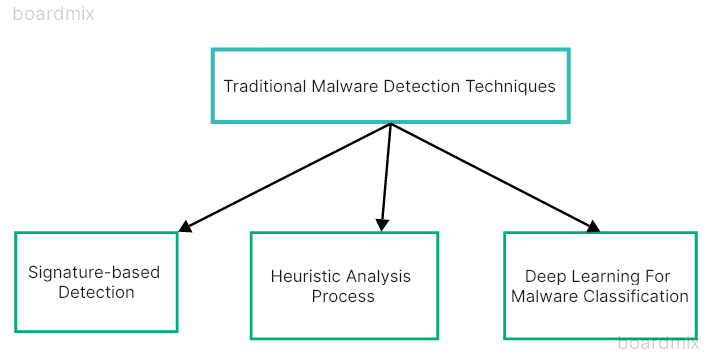
\includegraphics[width=0.5\textwidth]{Untitled.png} % Replace 'example-image' with your image filename
  \caption{Traditional Malware Detection Techniques } % Caption for the figure
  \label{fig:example2} % Label to refer to the figure in the text
\end{figure}



\subsection{Advantages of Deep Learning for Malware Classification}
\subsubsection{Signature-independence} Unlike signature-based detection, deep learning models do not require prior knowledge of specific malware signatures.
\subsubsection{New and unseen malware detection}
Can identify new malware variants based on patterns learned from training data.
\subsubsection{Reduced false positives} Deep learning models can potentially achieve higher accuracy and reduce false positives compared to heuristic analysis.


\section{Literature Review}
\subsection{Related Research}
Several studies have investigated the application of CNNs for malware classification, achieving promising results. For instance, the research by Mahamad Kalash et al. (2018) employed a deep CNN architecture with four convolutional layers and ReLU activation functions [1]. They trained the model on a dataset of malware samples converted into grayscale images using the Malimg dataset [15]. Their findings demonstrated an accuracy of 98.52\% in differentiating between various malware classes [1].

Another study by  Gibert et al. (2018) explored a different CNN architecture with three convolutional layers, utilizing techniques like global average pooling (GAP) and spatial pyramid pooling (SPP) [2]. Their research achieved a classification accuracy of 99.18\% on a dataset combining the Malimg dataset and a dataset collected from various sources [2]. These studies highlight the effectiveness of CNNs for malware classification, achieving high accuracy rates.

\subsection{Focus areas in existing research}
Existing research on CNN-based malware classification focuses on several key areas:

    CNN Architectures: Different CNN architectures have been explored, with variations in the number of convolutional layers, filter sizes, and activation functions. The research by Kalash et al. (2018) and Gibert et al. (2018) exemplifies this focus, demonstrating the effectiveness of both deep and shallower CNN architectures with different pooling techniques [1, 2].

    Pre-processing Techniques:  Pre-processing techniques play a crucial role in preparing malware samples for CNN input. Techniques like resizing, normalization, and conversion to specific formats (e.g., grayscale images) have been investigated. The study by Kalash et al. (2018) exemplifies this focus, converting malware samples into grayscale images before feeding them into the CNN model [1].

    Evaluation Metrics:  Evaluation metrics used to assess model performance include accuracy, precision, recall, and F1-score. While accuracy is a common metric, studies might utilize a combination of these metrics to provide a more comprehensive understanding of the model's performance.

\subsection{Our Work}
This work proposes a deep learning framework for malware image classification using transfer learning. We leverage pre-trained Convolutional Neural Networks (CNNs) to address the growing challenge of malware detection. Our approach builds upon existing research by:

    \textbf{Modular Framework}: We implement a modular pipeline for data exploration, preprocessing, model fine-tuning, experimentation, and evaluation. This facilitates adaptability and future enhancements.
    
    \textbf{Custom MalwareImages Class}: This class facilitates exploration of the malware image datasets, enabling visualization of class distribution and sample images for initial understanding.
    
    \textbf{Fine-Tuning with Early Stopping}: We employ a FineTuning class that fine-tunes pre-trained CNN architectures like XceptionNet. This class freezes initial layers, adds a final classification layer specific to malware categories, and trains the model with early stopping to optimize training efficiency.
    
    \textbf{Experimentation with Different CNNs}: The code allows experimentation with various pre-trained CNN models on individual and combined datasets. This enables us to assess the effectiveness of different architectures for malware image classification.

By leveraging transfer learning and establishing a modular framework, our work aims to contribute to the development of efficient and accurate malware detection systems using deep learning and image classification techniques.

\section{Methodology}
\subsection{Data Aquisition}
The data acquisition stage in our deep learning framework focuses on loading and exploring the blended malware image dataset.

\subsubsection{Dataset Selection}

    We leverage a publicly available blended malware image dataset from Kaggle. This dataset combines the Malimg and Malevis datasets, incorporating the advantages of both:
    
        Malimg Dataset: Contains byteplot images converted from Portable Executable (PE) files representing malware samples. However, it's known to have a highly imbalanced class distribution, meaning some malware types are more prevalent than others.
        
        Malevis Dataset: Also contains byteplot images of malware, but it's well-balanced in terms of class distribution, ensuring all malware types are represented more equally.
        
    The blended dataset offers a larger dataset with a more balanced class distribution compared to the individual datasets, making it suitable for training deep learning models.

\subsubsection{Data Loading}

    A custom MalwareImages class is utilized to load the blended dataset from Kaggle. 
    The MalwareImages class would handle tasks like:
        Downloading the dataset (if not already downloaded).
        Extracting the data from any compressed archive format (if applicable).

        Loading the image files and potentially associated labels (indicating the malware type for each image) into appropriate data structures within the code.

\subsubsection{Data Exploration}

    Once loaded, the MalwareImages class facilitates the exploration and visualization of the dataset to gain initial insights. This exploration might involve:
    
        Class Distribution Visualization: The class distribution within the blended dataset is visualized using techniques like bar charts or histograms. This helps us understand the prevalence of different malware categories and ensures all classes are represented more equally in the balanced dataset. It's important to note the number of samples per class at this stage.
        
        Sample Image Exploration: Sample images from various malware classes are displayed for initial exploration of the data. This visual inspection can reveal insights into the characteristics of the byteplot images and potential challenges for image classification. For instance, we might observe variations in image size, color depth (grayscale or RGB), or the level of detail within the images.

By exploring the data, we can gain a better understanding of the dataset's characteristics and potential issues that might require addressing during data preprocessing (e.g., handling class imbalance if present) or model training.


\subsection{Data Preprocessing}

\subsubsection{Resizing and Normalization}

    The ImageProcessor class resizes images to a specific size defined during its initialization. This ensures all images have a uniform input size for the CNN model.
    Normalization is applied within the data generator created by ImageProcessor. Normalization typically scales pixel values to a specific range (e.g., 0-1 or -1 to 1) to improve model convergence and stability.

\subsubsection{Data Augmentation}

    The code structure suggests the possibility of data augmentation techniques being used within the data generator. These techniques artificially create variations of existing images (e.g., random flips, rotations) to increase the training data size and improve model generalization.

    The ImageProcessor class handles color mode conversion based on the specified mode (e.g., RGB, grayscale). Converting images to a consistent color mode ensures the model processes the color information consistently.

\subsubsection{Data Generators}

    We utilize Keras's ImageDataGenerator class or a similar approach within ImageProcessor to create data generators for training, validation, and testing. These generators efficiently load, preprocess, and batch images during model training and evaluation.

\subsection{Model Selection and Fine Tuning}

    The code leverages pre-trained CNN architectures like XceptionNet. This model is a  powerful feature extractor trained on large image datasets.
    
    The FineTuning class facilitates fine-tuning these pre-trained models for the specific task of malware classification. Fine-tuning involves: 

    Selecting specific layers in the pre-trained model to be trainable again while keeping earlier layers frozen.
    Adding a final classification layer on top of the pre-trained model, potentially with regularization to prevent overfitting.

\subsection{Model Training}
The code utilizes a FineTuning class specifically designed for training CNN models for malware image classification using pre-trained architectures. Here's a breakdown of the model training process based on the code:



\subsubsection{Pre-trained Model Selection}

    A pre-trained CNN model XceptionNet. These models are loaded using libraries like TensorFlow or Keras.

\subsubsection{Fine-tuning Configuration}

    The FineTuning class allows specifying which layers in the pre-trained model to be marked as trainable. This is crucial for fine-tuning, as we want the model to adapt to the new classification task while leveraging the learned features from the pre-trained layers.

\subsubsection{Adding Final Classification Layer}

    The FineTuning class includes functionality to add a final classification layer on top of the pre-trained model. This layer has the number of neurons equal to the number of malware classes the model needs to predict.

\subsubsection{Regularization}

    The code might allow enabling regularization techniques (e.g., L1/L2 regularization, dropout) during the addition of the final layer. Regularization helps prevent overfitting by penalizing models with overly complex decision boundaries.

\subsubsection{Model Compilation}

    The FineTuning class compiles the model with the following elements:
        Optimizer: An optimizer (e.g., Adam) is specified to update the model's weights during training based on the calculated loss.
        
        Loss function: A loss function (e.g., categorical cross-entropy) is chosen to measure the model's performance on a single training example. This function guides the optimizer in adjusting the weights to minimize the loss.
        
        Metrics: Various metrics (e.g., accuracy, precision, recall) are defined to monitor the training progress and evaluate model performance on different aspects.

\subsubsection{Training with Early Stopping}

    The FineTuning class   facilitates training the model on the preprocessed training data generators. These generators efficiently load and feed batches of images to the model during training.
    Early stopping is implemented to prevent overfitting. This technique monitors the validation loss calculated on the validation data generator. If the validation loss doesn't improve for a certain number of epochs (iterations), training is terminated to avoid the model memorizing the training data instead of learning generalizable patterns.

\begin{figure}[ht] % 'h' stands for 'here', it tries to place the figure here
        \centering % Centers the figure horizontally
        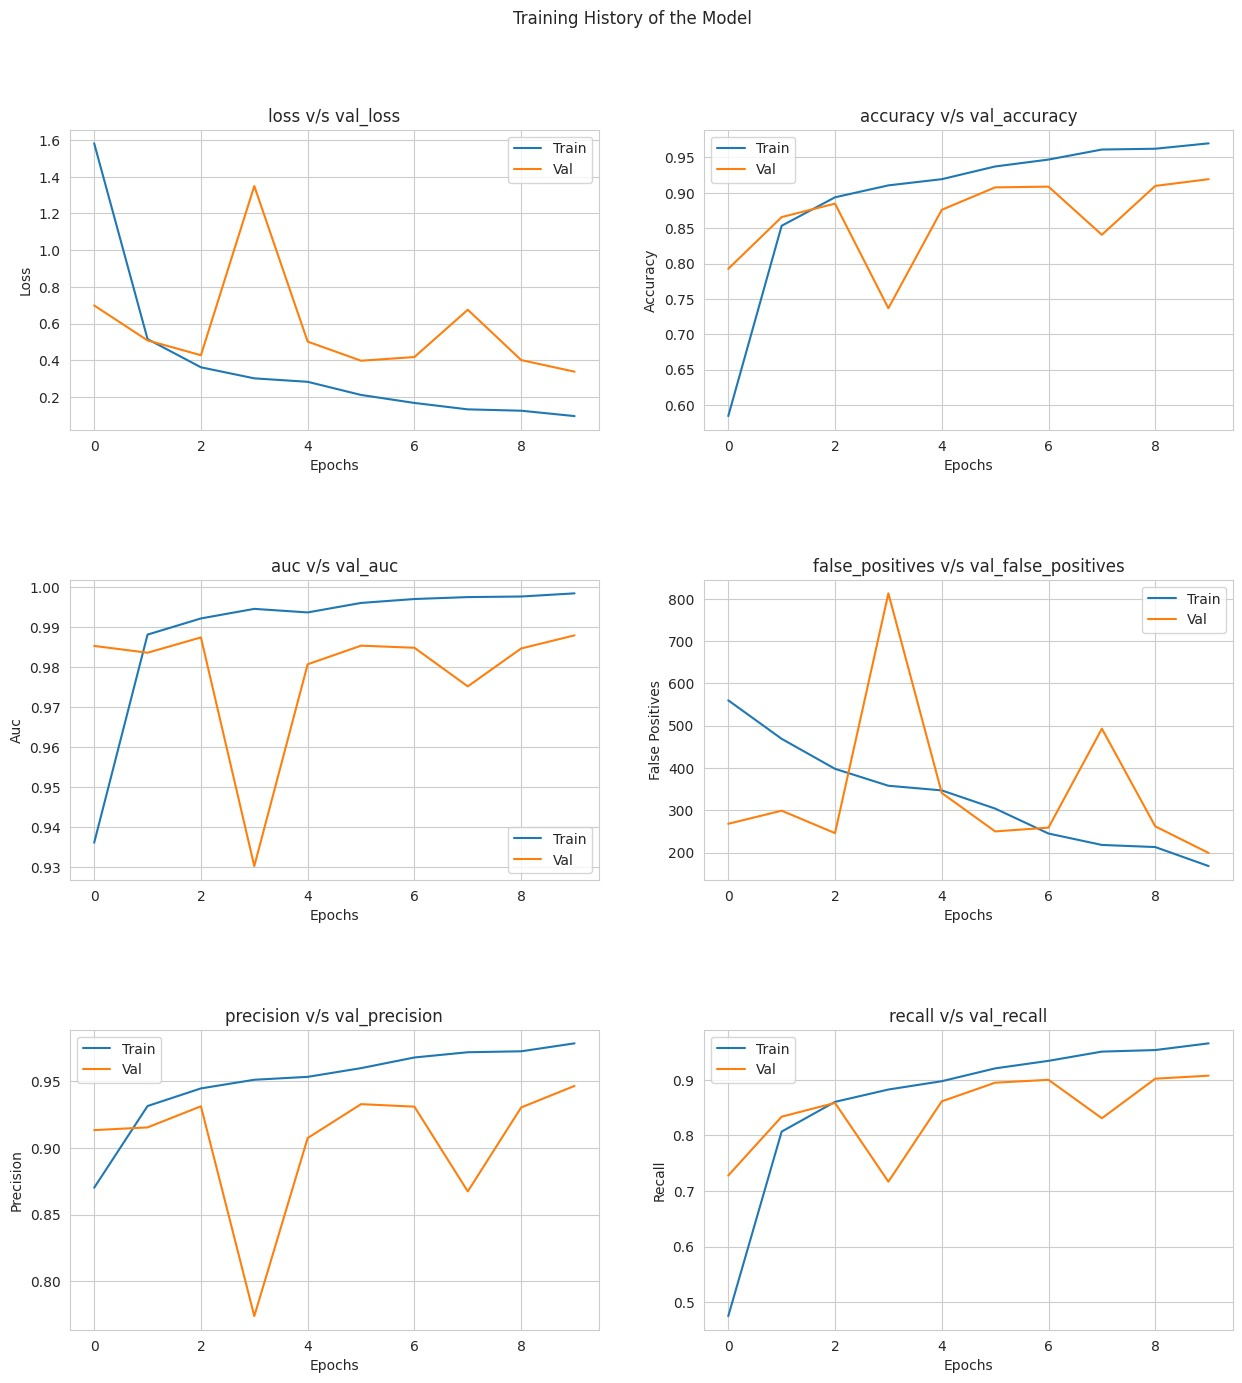
\includegraphics[width=0.5\textwidth]{training history.jpeg} % Replace 'example-image' with your image filename
        \caption{Model Training Results} % Caption for the figure
        \label{fig:example5} % Label to refer to the figure in the text
      \end{figure}
       
      As shown in Fig 3 the accuracy of the model increases as we increase the number of epochs, giving 97.13\% accuracy at around epoch 10, loss decreases to about 2\% by epoch 10, area under curve reaches 99.98 by epoch 10, false positives decrease to about 170 out of total input size of 10,000 images, the precision increases to around 97\% by epoch 10 and recall increases to 98\% as well by epoch 10.
\subsection{Model Evaluation}
We utilize a ModelEvaluator class specifically designed to evaluate the performance of CNN models trained for malware image classification. Here's a breakdown of the model evaluation process based on the code:

\subsubsection{Accessing Training History and Labels}

    The ModelEvaluator class  takes the model's training history as input. This history contains information about the loss and various metrics (accuracy, precision, recall) recorded during each training epoch.
    The class also receives the ground truth labels for the test data.

\subsubsection{Visualization of Training Process}

    The ModelEvaluator class  offers functionalities to plot the training history metrics (loss, accuracy) over epochs. These plots help visualize how the model's performance improved during training and identify potential issues like overfitting.

\subsubsection{Model Prediction on Test Data}

    The ModelEvaluator class uses the trained model to make predictions on the preprocessed test data generator. This generator efficiently feeds batches of test images to the model for prediction.

\subsubsection{Classification Report Generation}

    The ModelEvaluator class  calculates various evaluation metrics based on the model's predictions and the ground truth labels for the test data. These metrics include:
        
        Accuracy: Ratio of correctly classified samples to the total number of samples.
        
        Precision: Ratio of true positives (correctly predicted malware samples) to all predicted positive samples.
        
        Recall: Ratio of true positives (correctly predicted malware samples) to all actual malware samples in the test data.
        
        F1-score: Harmonic mean of precision and recall.
    
    The class  generates a classification report summarizing these metrics for each malware class the model predicts.

    \begin{figure}[h] % 'h' stands for 'here', it tries to place the figure here
        \centering % Centers the figure horizontally
        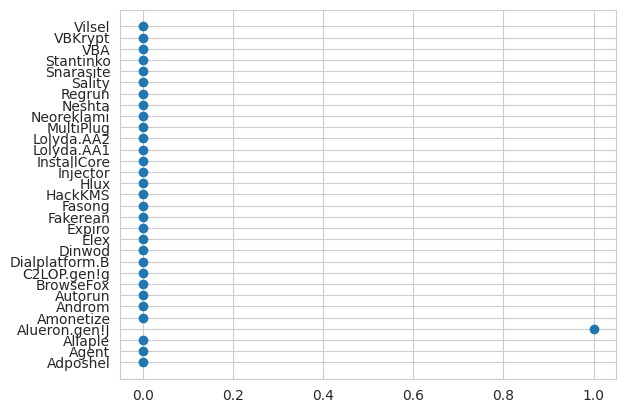
\includegraphics[scale=0.4]{PredictionResults.jpeg} % Replace 'example-image' with your image filename
        \caption{Prediction Results } % Caption for the figure
        \label{fig:example7} % Label to refer to the figure in the text
      \end{figure}


      Figure 4 shows the results of the model's predictions across all the various classes of malware, and it also shows desirable results, as it correctly identifies 30 out of the 31 classes.


\subsubsection{Confusion Matrix Generation}

    The ModelEvaluator class creates a confusion matrix to visualize the performance of the model for each class. The confusion matrix shows:
        
        True positives: Correctly classified malware samples for each class.
        
        False positives: Non-malware samples incorrectly classified as malware 
        for each class.

        False negatives: Malware samples incorrectly classified as non-malware.
        
        True negatives: Non-malware samples correctly classified.
    By analyzing the confusion matrix, researchers can identify potential biases or weaknesses in the model's performance for specific malware classes.
      \\
      \\
    Figure 5 page showcases the confusion matrix of the predictions, which show the number of false positives, true positives, false negatives and true negatives of the predictions across the 30 different classes of malware. We obtain desirable results, as the number of correct predictions, i.e. true positive and true negative across all the classes outnumber the false negatives and false positives.

\begin{figure}[ht] % 'h' stands for 'here', it tries to place the figure here
  \centering % Centers the figure horizontally
  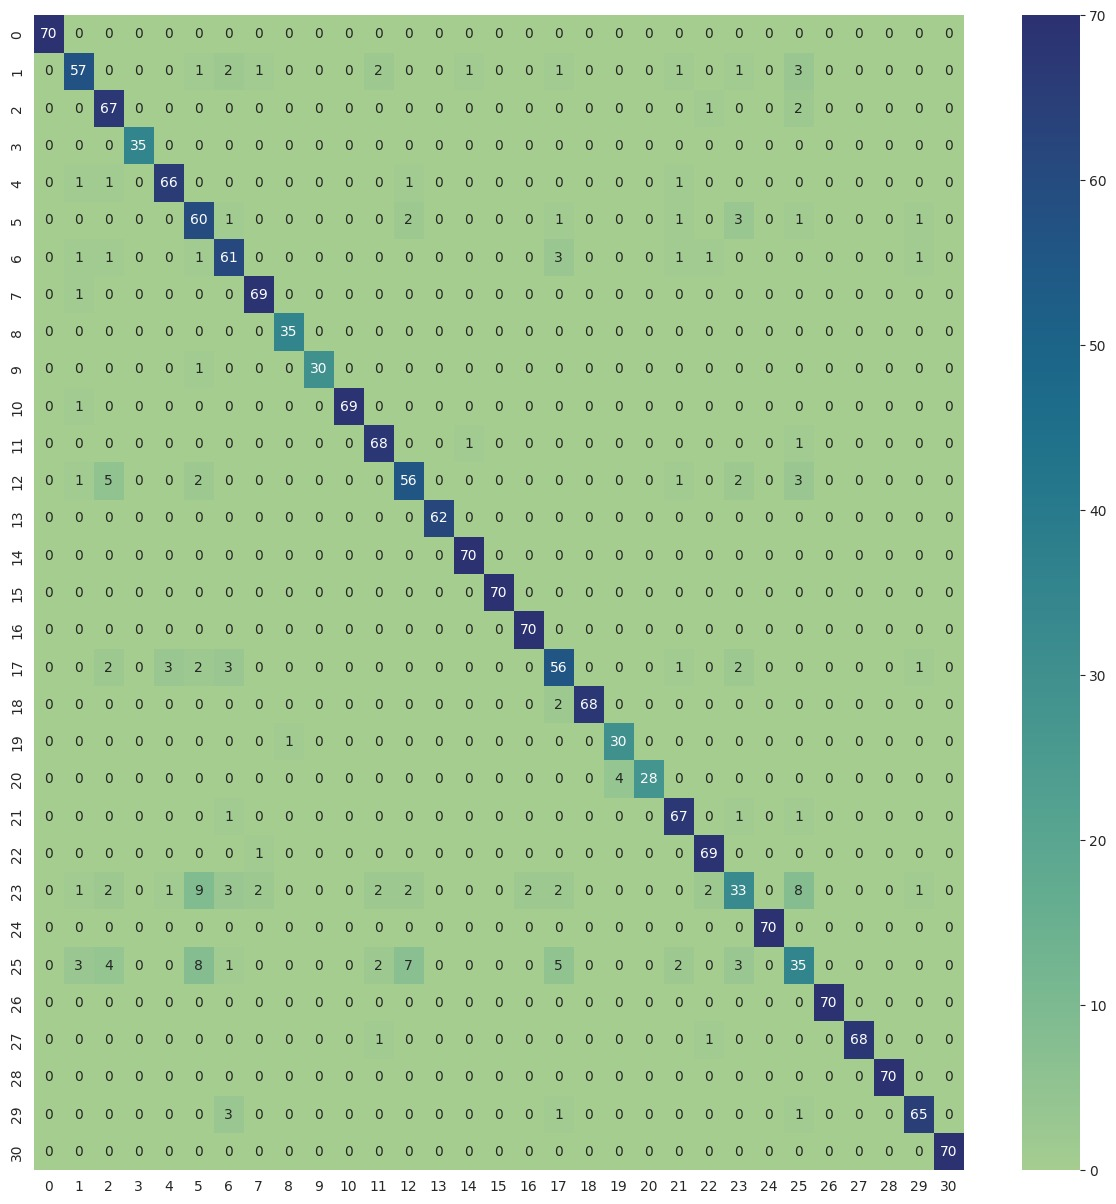
\includegraphics[width=0.5\textwidth]{confusionmatrixf.jpeg} % Replace 'example-image' with your image filename
  \caption{Confusion Matrix} % Caption for the figure
  \label{fig:example6} % Label to refer to the figure in the text
\end{figure}

\subsection{ Metrics}
The performance of the model will be evaluated using the following metrics:

    Accuracy: The overall percentage of correctly classified malware samples.
    
    Precision: The proportion of true positives (correctly identified malware) among all positive predictions.
    
    Recall: The proportion of true positives out of all actual malware samples.
    F1-score: A harmonic mean of precision and recall, providing a balanced measure of model performance.





% \begin{figure}[] % 'h' stands for 'here', it tries to place the figure here
%   \centering % Centers the figure horizontally
%   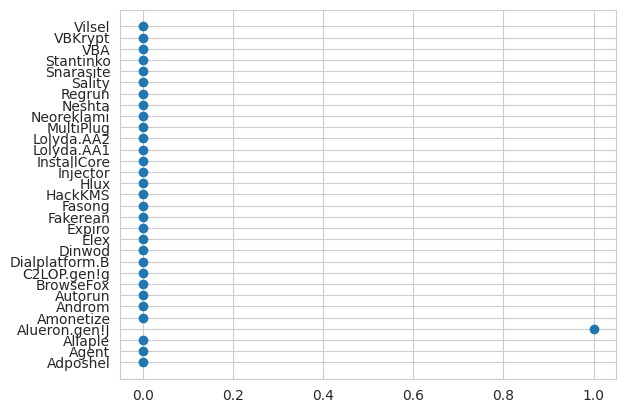
\includegraphics[scale=0.4]{PredictionResults.jpeg} % Replace 'example-image' with your image filename
%   \caption{Prediction Results } % Caption for the figure
%   \label{fig:example7} % Label to refer to the figure in the text
% \end{figure}

\setlength{\parskip}{10pt}

\subsection{Conclusion}
Our research highlights the potential of using Convolutional Neural Networks (CNNs) for malware classification, showing that they can outperform traditional antivirus software in terms of accuracy and speed. By training the CNN on grayscale images of malware samples, we were able to achieve results in identifying different types of malware. However, our study also pointed out some limitations, especially regarding the quality and diversity of the training data. To build on these findings, future work should explore more advanced CNN architectures, find ways to deal with class imbalances, and improve the model’s ability to recognize new, unseen malware. Additionally, making the model more robust against adversarial attacks will be crucial. These steps will help enhance the effectiveness of CNN-based approaches in combating evolving malware threats.

    
\begin{thebibliography}{00}
\bibitem{b1} Gibert, D., Mateu, C., Planes, J. et al. Using convolutional neural networks for classification of malware represented as
images. Using convolutional neural networks for classification of ... – Springer.

\bibitem{b2}Daniel Gibert, Carles Mateu, Jordi Planes, Journal of Network and Computer Applications, The rise of machine learning for detection and classification of malware: Research developments, trends and challenges. The rise of machine learning for detection and ... – ScienceDirect.
Daniel Gibert, Carles Mateu, Jordi Planes, Journal of Network and Computer Applications, The rise of machine learning for detection and classification of malware: Research developments, trends and challenges. The rise of machine learning for detection and ... – ScienceDirect.

\bibitem{b3}Songqing Yue, Tianyang Wang, Imbalanced Malware Images Classification: a CNN based Approach. Imbalanced Malware
Images Classification: a CNN based Approach.

\bibitem{b4}Nataraj, Lakshmanan, Karthikeyan, Shanmugavadivel, Jacob, Grégoire, Manjunath, B.. (2011). Malware Images: Visualization and Automatic Classification. 10.1145/2016904.2016908. Malware Images: Visualization and Automatic Classification – ResearchGate.

\bibitem{b5}M. Kalash, M. Rochan, N. Mohammed, N. D. B. Bruce, Y. Wang and F. Iqbal, "Malware Classification with Deep Convolutional Neural Networks," 2018 9th IFIP International Conference on New Technologies, Mobility and Security (NTMS), Paris, France, 2018, pp. 1-5, doi: 10.1109/NTMS.2018.8328749. Malware Classification with Deep Convolutional Neural Networks | IEEE ...

\bibitem{b6} Tuan, Anh Pham; Phuong, An Tran Hung; Thanh, Nguyen Vu; Van, Toan Nguyen (2018). Malware Detection PE-Based Analysis Using Deep Learning Algorithm Dataset. figshare. Dataset. Malware Detection PE-Based Analysis Using Deep Learning Algorithm Dataset.

\bibitem{b7} Conti, G. Bratus, S. Sangster, B. Ragsdale, S. Supan, M.
Lichtenberg, A. Perez, R. and Shubina, A. 2010. Automated
Mapping of Large Binary Objects Using Primitive Fragment Type
Classification Digital Forensics Research Conference (DFRWS)

\bibitem{b8} Falana, O.J., Sodiya, A.S., Onashoga, S.A. and Badmus, B.S., 2022. Mal-Detect: An intelligent visualization approach for malware detection. Journal of King Saud University-Computer and Information Sciences, 34(5), pp.1968-1983.

\bibitem{b9} AlGarni, M.D., AlRoobaea, R., Almotiri, J., Ullah, S.S., Hussain, S. and Umar, F., 2022. An efficient convolutional neural network with transfer learning for malware classification. Wireless Communications and Mobile Computing, 2022(1), p.4841741.

\bibitem{b10} Mourtaji, Y., Bouhorma, M. and Alghazzawi, D., 2019, March. Intelligent framework for malware detection with convolutional neural network. In Proceedings of the 2nd international conference on networking, information systems \& security (pp. 1-6).

\bibitem{b11} Anandhi, V., Vinod, P. and Menon, V.G., 2021. Malware visualization and detection using DenseNets. Personal and Ubiquitous Computing, pp.1-17.

\bibitem{b12} Abdullayeva, F., 2019, October. Malware detection in cloud computing using an image visualization technique. In 2019 IEEE 13th International Conference on Application of Information and Communication Technologies (AICT) (pp. 1-5). IEEE.

\bibitem{b13} Makandar, A. and Patrot, A., 2017, February. Malware class recognition using image processing techniques. In 2017 International Conference on Data Management, Analytics and Innovation (ICDMAI) (pp. 76-80). IEEE.

\bibitem{b14} Bensaoud, A., Abudawaood, N. and Kalita, J., 2020. Classifying malware images with convolutional neural network models. International Journal of Network Security, 22(6), pp.1022-1031.

\end{thebibliography}
\vspace{12pt}

\end{document}
